\documentclass[tikz, border=10pt]{standalone}
\usepackage{amsmath, amssymb}
\usetikzlibrary{matrix, positioning, fit, backgrounds, calc, shapes.geometric, arrows.meta}
\usepackage[T1]{fontenc}
\usepackage[utf8]{inputenc}
\usepackage{newpxtext,newpxmath}
\usepackage{sectsty}
\begin{document}
	
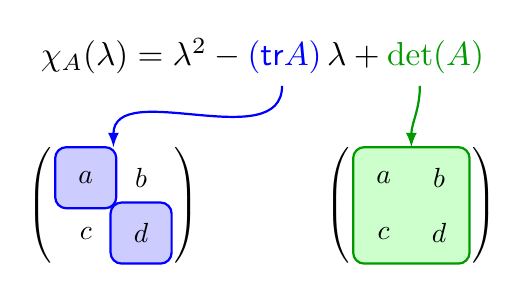
\begin{tikzpicture}[
	font=\sffamily,
	mtx/.style={
		matrix of math nodes,
		left delimiter=(, right delimiter=),
		nodes={minimum size=1.5em, anchor=center},
		column sep=5pt, row sep=5pt,
		ampersand replacement=\&
	},
	hl-trace/.style={fill=blue!20, draw=blue, thick, rounded corners},
	hl-det/.style={fill=green!20, draw=green!60!black, thick, rounded corners},
	arrow/.style={->, >=latex, thick, color=gray}
	]
	
	% Main Equation
	\node[scale=1.2] (eq) {$\chi_A(\lambda) = \lambda^2 - \textcolor{blue}{(\text{tr} A)}\,\lambda + \textcolor{green!60!black}{\det(A)}$};
	
	% Branch 1: Trace
	\node[below left=2.5] (trace_node) {};
	\matrix[mtx] (M_trace) at (trace_node) {
		a \& b \\
		c \& d \\
	};
	\begin{scope}[on background layer]
		\node[hl-trace, fit=(M_trace-1-1)] {};
		\node[hl-trace, fit=(M_trace-2-2)] {};
	\end{scope}
%	\node[below=0.2cm of M_trace, text=blue] {Sum of 1-Minors};
	
	% Branch 2: Determinant
	\node[below right=2.5] (det_node) {};
	\matrix[mtx] (M_det) at (det_node) {
		a \& b \\
		c \& d \\
	};
	\begin{scope}[on background layer]
		\node[hl-det, fit=(M_det-1-1)(M_det-2-2)] {};
	\end{scope}
%	\node[below=0.2cm of M_det, text=green!60!black] {2-Minor (Full)};
	
	% Arrows
	\draw[arrow, blue] ($(eq.south)+(.25,0)$) to[out=270, in=90] (M_trace.north);
	\draw[arrow, green!60!black] ($(eq.south)+(2,0)$) to[out=270, in=90] (M_det.north);
	
\end{tikzpicture}
	
	
%	\begin{tikzpicture}[
%		font=\sffamily,
%		% Style for the 3x3 matrices
%		mtx/.style={
%			matrix of math nodes,
%			left delimiter=(, right delimiter=),
%			nodes={minimum size=1.2em, inner sep=2pt, anchor=center},
%			column sep=2pt, row sep=2pt,
%			ampersand replacement=\&
%		},
%		% Highlighting styles
%		hl-trace/.style={fill=blue!20, draw=blue, thick, rounded corners=2pt},
%		hl-minor/.style={fill=orange!20, draw=orange, thick, rounded corners=2pt},
%		hl-det/.style={fill=green!20, draw=green!60!black, thick, rounded corners=2pt},
%		% Connector styles
%		arrow/.style={->, >=latex, thick, color=gray},
%		term label/.style={font=\bfseries\small, align=center}
%		]
%		
%		% --- 1. The Main Polynomial Equation ---
%		\node[scale=1.2] (eq) at (0, 0) {
%			$\chi_A(t) = -t^3 + \textcolor{blue}{c_2} t^2 - \textcolor{orange}{c_1} t + \textcolor{green!60!black}{c_0}$
%		};
%		
%		% --- 2. Coefficient Visualizations (Branches) ---
%		
%		% === Branch 1: Trace (c2) ===
%		\node[below=2cm of eq, xshift=-5cm] (trace_node) {};
%		% We use a single matrix to show the diagonal
%		\matrix[mtx] (M_trace) at (trace_node) {
%			a \& b \& c \\
%			d \& e \& f \\
%			g \& h \& i \\
%		};
%		% Highlight Diagonal
%		\begin{scope}[on background layer]
%			\node[hl-trace, fit=(M_trace-1-1)] {};
%			\node[hl-trace, fit=(M_trace-2-2)] {};
%			\node[hl-trace, fit=(M_trace-3-3)] {};
%		\end{scope}
%		\node[below=0.2cm of M_trace, term label, text=blue] (lbl_trace) {Sum of 1-Minors\\(Trace)};
%		\node[below=0mm of lbl_trace, scale=0.8] {$a + e + i$};
%		
%		% === Branch 2: Sum of 2-Minors (c1) ===
%		% We need 3 small matrices to show the 3 principal minors
%		\node[below=2cm of eq] (minor_node) {};
%		
%		% Minor {1,2} (Top Left)
%		\matrix[mtx, scale=0.8] (M_m1) at ($(minor_node)+(-2.2, 0)$) {
%			a \& b \& c \\
%			d \& e \& f \\
%			g \& h \& i \\
%		};
%		\begin{scope}[on background layer]
%			\node[hl-minor, fit=(M_m1-1-1)(M_m1-2-2)] {}; 
%		\end{scope}
%		\node[below=0.1cm of M_m1, scale=0.7] {$\det\binom{a\,b}{d\,e}$};
%		
%		% Minor {2,3} (Bottom Right)
%		\matrix[mtx, scale=0.8] (M_m2) at (minor_node) {
%			a \& b \& c \\
%			d \& e \& f \\
%			g \& h \& i \\
%		};
%		\begin{scope}[on background layer]
%			\node[hl-minor, fit=(M_m2-2-2)(M_m2-3-3)] {};
%		\end{scope}
%		\node[below=0.1cm of M_m2, scale=0.7] {$\det\binom{e\,f}{h\,i}$};
%		
%		% Minor {1,3} (Corners) - The tricky one
%		\matrix[mtx, scale=0.8] (M_m3) at ($(minor_node)+(2.2, 0)$) {
%			a \& b \& c \\
%			d \& e \& f \\
%			g \& h \& i \\
%		};
%		\begin{scope}[on background layer]
%			% Highlight the 4 corners involved
%			\node[hl-minor, fit=(M_m3-1-1)] {};
%			\node[hl-minor, fit=(M_m3-1-3)] {};
%			\node[hl-minor, fit=(M_m3-3-1)] {};
%			\node[hl-minor, fit=(M_m3-3-3)] {};
%			% Connect them visually
%			\draw[orange, opacity=0.3, line width=3pt] (M_m3-1-1.center) -- (M_m3-1-3.center) -- (M_m3-3-3.center) -- (M_m3-3-1.center) -- cycle;
%		\end{scope}
%		\node[below=0.1cm of M_m3, scale=0.7] {$\det\binom{a\,c}{g\,i}$};
%		
%		\node[below=1.2cm of minor_node, term label, text=orange] (lbl_minor) {Sum of 2-Minors};
%		
%		
%		% === Branch 3: Determinant (c0) ===
%		\node[below=2cm of eq, xshift=5cm] (det_node) {};
%		\matrix[mtx] (M_det) at (det_node) {
%			a \& b \& c \\
%			d \& e \& f \\
%			g \& h \& i \\
%		};
%		\begin{scope}[on background layer]
%			\node[hl-det, fit=(M_det-1-1)(M_det-3-3)] {};
%		\end{scope}
%		\node[below=0.2cm of M_det, term label, text=green!60!black] (lbl_det) {3-Minor\\(Determinant)};
%		\node[below=0mm of lbl_det, scale=0.8] {$\det(A)$};
%		
%		
%		% --- 3. Arrows and Annotations ---
%		
%		% Arrow to Trace
%		\draw[arrow, blue] ($(eq.south)+(-1.5,0)$) to[out=270, in=90] node[midway, left, font=\scriptsize] {Coefficient of $t^2$} (M_trace.north);
%		
%		% Arrow to Minors
%		\draw[arrow, orange] (eq.south) to[out=270, in=90] node[midway, fill=white, inner sep=1pt, font=\scriptsize] {Coefficient of $-t^1$} (M_m2.north);
%		
%		% Arrow to Det
%		\draw[arrow, green!60!black] ($(eq.south)+(1.5,0)$) to[out=270, in=90] node[midway, right, font=\scriptsize] {Constant Term} (M_det.north);
%		
%		% Plus signs between the minors
%		\node at ($(M_m1)!0.5!(M_m2)$) {$+$};
%		\node at ($(M_m2)!0.5!(M_m3)$) {$+$};
%		
%	\end{tikzpicture}
%
%	\begin{tikzpicture}[
%		font=\sffamily,
%		mtx/.style={
%			matrix of math nodes,
%			left delimiter=(, right delimiter=),
%			nodes={minimum size=1.1em, inner sep=1pt, anchor=center},
%			column sep=2pt, row sep=2pt,
%			ampersand replacement=\&
%		},
%		% Styles for different levels of minors
%		hl-1/.style={fill=blue!20, draw=blue, thick},                 % Trace
%		hl-2/.style={fill=orange!20, draw=orange, thick},             % 2x2
%		hl-3/.style={fill=purple!20, draw=purple, thick},             % 3x3
%		hl-4/.style={fill=green!20, draw=green!60!black, thick},      % Det
%		arrow/.style={->, >=latex, thick, color=gray!80},
%		label/.style={font=\scriptsize\bfseries, align=center, inner sep=2pt}
%		]
%		
%		% --- Top Equation ---
%		\node[scale=1.1] (eq) at (0,0) {
%			$\chi_A(t) = t^4 - \textcolor{blue}{c_3} t^3 + \textcolor{orange}{c_2} t^2 - \textcolor{purple}{c_1} t + \textcolor{green!60!black}{c_0}$
%		};
%		
%		% --- Level 1: Trace (c3) ---
%		\node[below left=2.5cm and 4.5cm of eq] (pos1) {};
%		\matrix[mtx] (M1) at (pos1) {
%			a \& \cdot \& \cdot \& \cdot \\
%			\cdot \& f \& \cdot \& \cdot \\
%			\cdot \& \cdot \& k \& \cdot \\
%			\cdot \& \cdot \& \cdot \& p \\
%		};
%		\begin{scope}[on background layer]
%			\node[hl-1, fit=(M1-1-1)] {};
%			\node[hl-1, fit=(M1-2-2)] {};
%			\node[hl-1, fit=(M1-3-3)] {};
%			\node[hl-1, fit=(M1-4-4)] {};
%		\end{scope}
%		\node[below=0.1cm of M1, text=blue, label] (L1) {Sum of 1-Minors\\(Trace)};
%		\node[below=0mm of L1, font=\tiny] {$\binom{4}{1}=4$ terms};
%		
%		
%		% --- Level 2: 2x2 Minors (c2) ---
%		\node[below left=2.5cm and 1.5cm of eq] (pos2) {};
%		\matrix[mtx] (M2) at (pos2) {
%			a \& b \& \cdot \& \cdot \\
%			e \& f \& \cdot \& \cdot \\
%			\cdot \& \cdot \& \cdot \& \cdot \\
%			\cdot \& \cdot \& \cdot \& \cdot \\
%		};
%		\begin{scope}[on background layer]
%			% Visualizing one example: The top-left 2x2
%			\node[hl-2, fit=(M2-1-1)(M2-2-2), inner sep=-1pt] {};
%		\end{scope}
%		% Stack effect to imply multiple terms
%		\begin{scope}[on background layer]
%			\draw[fill=white, draw=gray!30] ($(M2.north west)+(2pt,2pt)$) rectangle ($(M2.south east)+(2pt,2pt)$);
%			\draw[fill=white, draw=gray!30] ($(M2.north west)+(1pt,1pt)$) rectangle ($(M2.south east)+(1pt,1pt)$);
%		\end{scope}
%		
%		\node[below=0.1cm of M2, text=orange, label] (L2) {Sum of 2-Minors};
%		\node[below=0mm of L2, font=\tiny] {$\binom{4}{2}=6$ terms};
%		
%		
%		% --- Level 3: 3x3 Minors (c1) ---
%		\node[below right=2.5cm and 1.5cm of eq] (pos3) {};
%		\matrix[mtx] (M3) at (pos3) {
%			a \& b \& c \& \cdot \\
%			e \& f \& g \& \cdot \\
%			i \& j \& k \& \cdot \\
%			\cdot \& \cdot \& \cdot \& \cdot \\
%		};
%		\begin{scope}[on background layer]
%			% Visualizing one example: Top-left 3x3
%			\node[hl-3, fit=(M3-1-1)(M3-3-3), inner sep=-1pt] {};
%		\end{scope}
%		% Stack effect
%		\begin{scope}[on background layer]
%			\draw[fill=white, draw=gray!30] ($(M3.north west)+(2pt,2pt)$) rectangle ($(M3.south east)+(2pt,2pt)$);
%			\draw[fill=white, draw=gray!30] ($(M3.north west)+(1pt,1pt)$) rectangle ($(M3.south east)+(1pt,1pt)$);
%		\end{scope}
%		
%		\node[below=0.1cm of M3, text=purple, label] (L3) {Sum of 3-Minors};
%		\node[below=0mm of L3, font=\tiny] {$\binom{4}{3}=4$ terms};
%		
%		
%		% --- Level 4: Determinant (c0) ---
%		\node[below right=2.5cm and 4.5cm of eq] (pos4) {};
%		\matrix[mtx] (M4) at (pos4) {
%			a \& b \& c \& d \\
%			e \& f \& g \& h \\
%			i \& j \& k \& l \\
%			m \& n \& o \& p \\
%		};
%		\begin{scope}[on background layer]
%			\node[hl-4, fit=(M4-1-1)(M4-4-4)] {};
%		\end{scope}
%		\node[below=0.1cm of M4, text=green!60!black, label] (L4) {4-Minor\\(Determinant)};
%		\node[below=0mm of L4, font=\tiny] {$\binom{4}{4}=1$ term};
%		
%		
%		% --- Arrows ---
%		\draw[arrow, blue] ($(eq.south)+(-3,0)$) to[out=270, in=90] (M1.north);
%		\draw[arrow, orange] ($(eq.south)+(-1,0)$) to[out=270, in=90] (M2.north);
%		\draw[arrow, purple] ($(eq.south)+(1,0)$) to[out=270, in=90] (M3.north);
%		\draw[arrow, green!60!black] ($(eq.south)+(3,0)$) to[out=270, in=90] (M4.north);
%		
%	\end{tikzpicture}
%
%\begin{tikzpicture}[
%	font=\sffamily,
%	% General matrix style with dots
%	mtx/.style={
%		matrix of math nodes,
%		left delimiter=(, right delimiter=),
%		nodes={minimum size=1.5em, anchor=center},
%		column sep=4pt, row sep=4pt,
%		ampersand replacement=\&
%	},
%	% Highlighting styles
%	hl-trace/.style={fill=blue!15, draw=blue, thick, rounded corners},
%	hl-general/.style={fill=orange!15, draw=orange, thick, rounded corners},
%	hl-det/.style={fill=green!15, draw=green!60!black, thick, rounded corners},
%	arrow/.style={->, >=latex, thick, color=gray!80},
%	label/.style={font=\small\bfseries, align=center}
%	]
%	
%	% --- Top Equation ---
%	\node[scale=1.1] (eq) at (0,0) {
%		$\chi_A(t) = \dots + (-1)^k \Bigl( \textcolor{orange}{\sum \det(A_{I})} \Bigr) t^{n-k} + \dots$
%	};
%	
%	% --- Branch 1: k=1 (Trace) ---
%	\node[below left=3cm and 5cm of eq] (pos1) {};
%	\matrix[mtx] (M1) at (pos1) {
%		a_{11} \& \dots \& \dots \& \dots \\
%		\vdots \& a_{22} \& \dots \& \vdots \\
%		\vdots \& \vdots \& \ddots \& \vdots \\
%		\dots \& \dots \& \dots \& a_{nn} \\
%	};
%	\begin{scope}[on background layer]
%		% Highlight diagonal elements abstractly
%		\node[hl-trace, fit=(M1-1-1)] {};
%		\node[hl-trace, fit=(M1-2-2)] {};
%		\node[hl-trace, fit=(M1-4-4)] {};
%	\end{scope}
%	\node[below=0.2cm of M1, text=blue, label] (L1) {k=1 (Trace)};
%	\node[below=0mm of L1, font=\tiny, align=center] {Sum of $\binom{n}{1}$ terms\\(Diagonal Sum)};
%	
%	
%	% --- Branch 2: General k (Principal Minors) ---
%	\node[below=3cm of eq] (pos2) {};
%	\matrix[mtx] (M2) at (pos2) {
%		a_{11} \& \dots \& \dots \& \dots \\
%		\vdots \& \mathbf{A}_{II} \& \dots \& \vdots \\
%		\vdots \& \dots \& \ddots \& \vdots \\
%		\dots \& \dots \& \dots \& a_{nn} \\
%	};
%	\begin{scope}[on background layer]
%		% Abstract selection of a k x k submatrix
%		\node[hl-general, fit=(M2-2-2)(M2-3-3), inner sep=5pt, label={[orange, font=\tiny]center:Submatrix of size $k$}] {};
%	\end{scope}
%	
%	\node[below=0.2cm of M2, text=orange, label] (L2) {General $k$};
%	\node[below=0mm of L2, font=\tiny, align=center] {Sum of $\binom{n}{k}$ Principal Minors\\(Size $k \times k$)};
%	
%	
%	% --- Branch 3: k=n (Determinant) ---
%	\node[below right=3cm and 5cm of eq] (pos3) {};
%	\matrix[mtx] (M3) at (pos3) {
%		a_{11} \& \dots \& \dots \& a_{1n} \\
%		\vdots \& \ddots \& \dots \& \vdots \\
%		\vdots \& \dots \& \ddots \& \vdots \\
%		a_{n1} \& \dots \& \dots \& a_{nn} \\
%	};
%	\begin{scope}[on background layer]
%		\node[hl-det, fit=(M3-1-1)(M3-4-4)] {};
%	\end{scope}
%	\node[below=0.2cm of M3, text=green!60!black, label] (L3) {k=n (Determinant)};
%	\node[below=0mm of L3, font=\tiny, align=center] {Single $\binom{n}{n}=1$ term\\(Full Matrix)};
%	
%	
%	% --- Arrows ---
%	% Trace Arrow
%	\draw[arrow, blue] ($(eq.south)+(-3,0)$) to[out=270, in=90] 
%	node[pos=0.6, left, font=\scriptsize] {Coeff of $t^{n-1}$} (M1.north);
%	
%	% General Arrow
%	\draw[arrow, orange] (eq.south) -- (M2.north);
%	\node[text=orange, font=\scriptsize, fill=white] at ($(eq.south)!0.5!(M2.north)$) {Coeff of $t^{n-k}$};
%	
%	% Det Arrow
%	\draw[arrow, green!60!black] ($(eq.south)+(3,0)$) to[out=270, in=90] 
%	node[pos=0.6, right, font=\scriptsize] {Constant Term ($t^0$)} (M3.north);
%	
%\end{tikzpicture}
	
\end{document}